\chapter{Method}%
\label{ch:method}

\newthought{In this chapter}, we introduce the theoretical idea of our Bayesian modelling of source separation. First, we explicitly state our chosen model of the problem, next derive a suitable optimization objective from it and then explain how we can optimize towards that.

We propose the graphical model as shown in \cref{fig:graphical_model} as the generative story of music tracks being generated from separate source tracks. For each source a sample is taken from the latent source distribution. The observed mix is generated deterministically from the full set of sources. Without loss of generality, we fix this function to be the mean.

\begin{marginfigure}[-15em]
    \begin{tikzpicture}
    \node[obs]                (x) {\(\x\)};
    \node[latent, left=of x]  (z) {\(\z\)};

    \edge {z} {x} ; %

    \plate {xz} {(x)(z)} {\(N\)} ;
\end{tikzpicture}
%
    \caption{The used graphical model for the source separation task. We have the latent source channel variables \(\s_k\). Exemplary here, as in our data, we have four sources. The mix \(\m\) is observed.}%
    \label{fig:graphical_model}
\end{marginfigure}

Our stated task in \sref{ch:question} is to retreive the sources \(\{\s_1,\…,\s_N\}\) from a given mix \(\m\). Our model is trained without using sample tuples \[(\m, \{\s_1,\…,\s_N\}): f(\{\s_1,\…,\s_N\}) = \m\] which would show the relation between separate sources and mixes. The general idea is visualized in \cref{fig:method}.

\begin{figure}[t]
    \begin{tikzpicture}
    % Data column
    \node                  (s0) {\includegraphics[width=25pt]{mixing/bass.png}};
    \node[below=0pt of s0] (s1) {\includegraphics[width=25pt]{mixing/drums.png}};
    \node[below=0pt of s1] (s2) {\includegraphics[width=25pt]{mixing/voice.png}};
    \node[below=0pt of s2] (s3) {\includegraphics[width=25pt]{mixing/other.png}};

    % Prior column
    \node[right=50pt of s0] (d0) {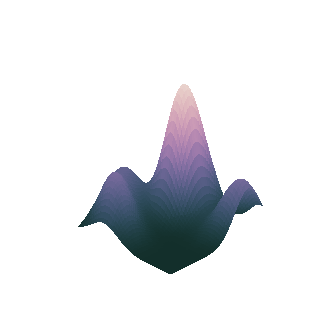
\includegraphics[width=40pt]{dist_0}};
    \node[right=50pt of s1] (d1) {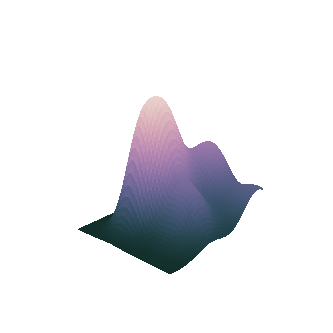
\includegraphics[width=40pt]{dist_1}};
    \node[right=50pt of s2] (d2) {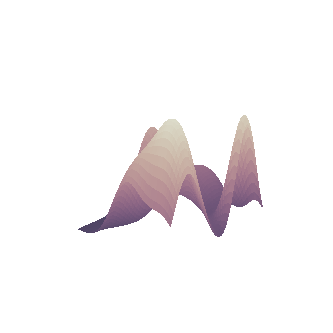
\includegraphics[width=40pt]{dist_2}};
    \node[right=50pt of s3] (d3) {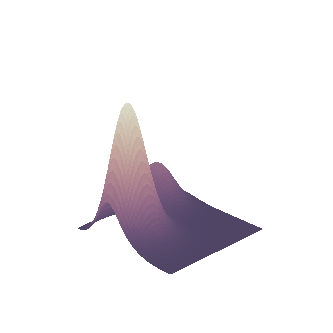
\includegraphics[width=40pt]{dist_3}};

    % Data to prior arrows
    \draw[->] (s0) to (d0);
    \draw[->] (s1) to (d1);
    \draw[->] (s2) to (d2);
    \draw[->] (s3) to (d3);

    % Posterior column
    \node[right=20pt of d0] (dp0) {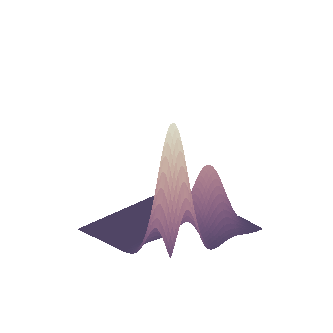
\includegraphics[width=40pt]{dist_0_post}};
    \node[right=20pt of d1] (dp1) {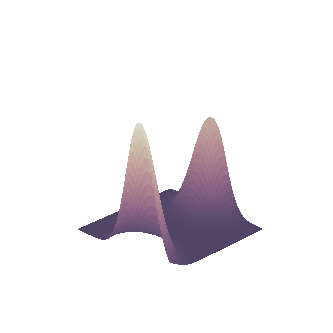
\includegraphics[width=40pt]{dist_1_post}};
    \node[right=20pt of d2] (dp2) {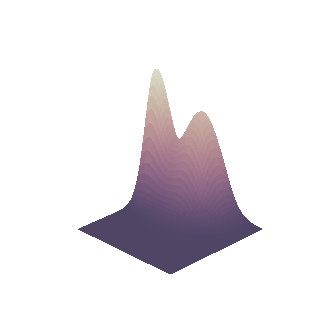
\includegraphics[width=40pt]{dist_2_post}};
    \node[right=20pt of d3] (dp3) {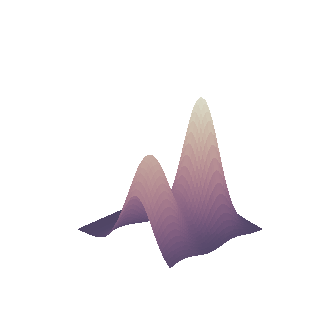
\includegraphics[width=40pt]{dist_3_post}};

    % Sample column
    \node[right=30pt of dp0] (ps0) {\includegraphics[width=30pt]{wave_bass}};
    \node[right=30pt of dp1] (ps1) {\includegraphics[width=30pt]{wave_drums}};
    \node[right=30pt of dp2] (ps2) {\includegraphics[width=30pt]{wave_voice}};
    \node[right=30pt of dp3] (ps3) {\includegraphics[width=30pt]{wave_other}};

    % Arrows from posterior to samples
    \draw[->] (dp0) to (ps0);
    \draw[->] (dp1) to (ps1);
    \draw[->] (dp2) to (ps2);
    \draw[->] (dp3) to (ps3);

    % Top row, notes
    \node[above=0pt of s0]   (ts)  {\(\D_k\)};
    \node[above=-9pt of d0]  (td)  {\(p_{\B{\θ}}(\s_k)\)};
    % \path (ts) -- (td) node [midway,align=center] {estimate\\with flow};
    \node[above=-9pt of dp0] (tdp) {\(\aprxpost\)};
    \node[above=0pt of ps0]  (tps) {\(\s_k\)};

    % Top top row
    \node[above=0pt of ts]  () {data};
    \node[above=0pt of td]  () {prior};
    \node[above=0pt of tdp] () {posterior};
    \node[above=0pt of tps] () {sample};

    % Mix wave
    \node[right=5pt of ps1, yshift=-20pt] (sum) {\(+\)};
    \node[right=-8pt of sum] (wav) {\includegraphics[width=30pt]{wave_mix}};

    \draw (ps0) -| (sum)
          (ps1) -| (sum)
          (ps2) -| (sum)
          (ps3) -| (sum);

    % Langevin
    \draw[->, bend angle=45, bend right=40]  ([yshift=-5pt]d3) to node[below] {sampling} node[above] {Langevin} ([yshift=-12pt,xshift=-10pt]ps3);
\end{tikzpicture}

    \caption{The method visualized}%
    \label{fig:method}%
    \setfloatalignment{b}%
\end{figure}

Looking back at the graphical model in \cref{fig:graphical_model}, it implies the following factorization:

\begin{align}
    p(\m)
    &= \∫^N p(\s_1,\…,\s_N,\m) \,d^N \s\\
    &= \∫^N p(\m | \s_1,\…,\s_N) \· p(\s_1,\…,\s_N) \,d^N \s\\
    &= \∫^N p(\m | \s_1,\…,\s_N) \· p(\s_1) \cdots p(\s_N) \,d^N \s
\end{align}

While the conditional \(p(\m | \s_1,\…,\s_N)\) is not even probabilistic, as the mix is generated deterministically as the mean of the sources, the model posterior \(p(\s_1,\…,\s_N | \m)\) is intractable and precisely what we are interested in. Again we want to make it clear that this setup changes the typical optimization target, as seen in other source separation approaches. We factorize the distribution \(p(\m)\) of mixed songs, only then to extract the most likely \I{latent} components that generate this mix, the sources. Therefore we are explicitly modelling the generative process of the mixed songs, and only implicitly the separation task.

Already with the graphical model we introduce a fairly big assumption, namely that we can model the source distributions independently from each other when modeling the joint:

\begin{align}
    p(\m,\s_1,\…,\s_N) &\equiv p(\m|\s_1,\…,\s_N) \· \Π_k^N p(\s_k)\label{eq:assumption}
\end{align}

Intuitively this assumption does not, in general, hold for the musical domain. We can expect a different behaviour for a \I{guitar} in a song involving a second source like a \I{percussion set}. The joint of those two models is different than their independent densities~\footnote{A practical counter-example: If learning the behaviour of drums, only from solo drum recordings, one will encounter complex rhythms and sounds. In many rock genres drums often exhibit simpler sounds, providing beat and tempo. These two distributions are not the same.}. Nevertheless, this assumption is crucial to be able to model the prior instrumental models without needing the tuples \((\s_1,\…,\s_N)\) of co-occurring stems.

The general process is as follows:

First, because we assumed in our graphical model the latent sources to be independent, there exists a probability distribution \(p(\s_k)\) for each source \(k\). Thereout we need to choose a model which gives the parametrized approximated prior \(p_{\B{\θ}}(\s_k)\) with the parameters \(\B{\θ}\) which we optimize with the samples from \(\mathcal{D}_k\).

Second, for each source, there exists a posterior given a mix \(p(\s_k | \m)\) from which we want to draw samples. Here two approaches are possible. Either we can propose an approximate posterior \(\aprxpost\), which is trained to minimize the divergence from the previously trained and fixed corresponding prior (VAE setting). Or, we can sample directly from the posterior using Stochastic Gradient Langevin Dynamics (SGLD)~\cite{wellingBayesian2011} without explicitly approximating the posterior distribution (sampling setting). Both optimization, either training or sampling, happen under the mixing constraint:

\begin{align}
    \Σ_{k=1}^N \s_k = \m
\end{align}

When using the VAE setting we then can sample from each posterior to retrieve a set of (approximately) correct source tracks. In the case of using Langevin dynamics, the iterative sampling will directly give this set from the prior distributions.

Thinking in the common terms of the VAE we need to choose:

\begin{enumerate}
    \item a parametrization \(p_{\B{\θ}}(\s_k)\) of the \I{prior} distribution
    \item a parametrized approximate posterior distribution \(\aprxpost\) with parameters \(\B{\η}\)
    \item a parametrized \I{encoder} which gives the parameters for the posterior distribution \(\texttt{Encoder}_{\B{\φ}}(\m) = \B{\η}\)
    \item a \I{decoder} which returns the input \(\m\) from the latents \linebreak \({\texttt{Decoder}(\{\s_1,\…,\s_N\}) = \m}\)
\end{enumerate}

As stated before the decoder in our case is the mean function, thus not probabilistic and without parameters. It is certainly possible to parametrize the decoder with trainable parameters. This would imply though that the latent samples are not in the \I{direct form} of the source sounds but under an (unknown) transformation.

\section{Modeling the priors}
The first step in the training procedure is the training of the independent source priors \(p(\s_k)\). We have to choose a model for estimating the density that results in smooth, tight densities but also is capable enough to capture the complex data space of audio data. We choose to estimate the priors with flow models for which we gave an overview in \sref{subsec:flows}. For different representations of the input, different network architectures are more suited. We experiment both with using directly the time-domain wave but also modelling on top of a spectral transformation of the time-domain data.

The two main variants of normalizing flows we build our priors from are the RealNVP and Glow. Their most important difference is the different formulation of the coupling layers. For the coupling layers, we have to split the layer input into two equally sized subsets, one of whom will be transformed using an invertible transformation parametrized by the other. The RealNVP masks the data spatially or over the channels. When done spatially a checkerboard binary mask is used (same for all channels), for the channel variant the channels are assigned in an even-odd switching. Glow, on the other hand, learns a \(1\× 1\)-convolution which permutes the data channel-wise and than just splits the data along the channel dimension into two. For both RealNVP and Glow prior work exists specifically adapting the architecture to the time-series domain by integrating WaveNet modules, FloWaveNet~\cite{kimFloWaveNet2019a} and WaveGlow~\cite{prengerWaveGlow2018}, respectively.

For the case of the time-domain representation, the data has only one channel (mono-audio). Therefore a Glow-like shuffling of channels is not possible and we resort to using spatial masking for the coupling layers. A one-dimensional mask is used over the time dimension. In the case of using a spectral representation of the audio data, the input samples have a lower time resolution but instead the frequency distribution over a deeper channel dimension. Therefore we can also experiment with channel-shuffling.

We make it clear that the success of this method depends strongly on the expressiveness and smoothness of the learned prior models. In the case of learning the posterior, variational learning will fit the posterior distribution under the prior distribution. If the prior does not contain enough variation of the actual data distribution, the de-mixing model cannot fit a conditional posterior similar to the sample in the mixed song. In the case of the sampling approach, this constraint is even more stressed. The mixed is generated by iteratively sampling from the set of prior distributions, any possible source sample, therefore, has to be found on the manifold of the prior. If any of the priors does not capture the full variations of the data distributions, neither method will be able to extract the correct separated sources.

More practically we again point out the high difficulty of modelling audio data. As laid out in \sref{subsec:audio} audio consists of information at greatly different resolutions. A generative model of an instrument has to model the low-range components, e.g.\ pitch, timbre, tremolo and high-range components, e.g.\ notes and rhythm.

\itodo{explain how prior actually looks like}

\section{Sampling from the posteriors}
After having estimated the \(N\) prior distributions the first possibility for retrieving sample estimates \(\s_k\) is sampling from the posterior using Langevin dynamics~\cite{wellingBayesian2011}. With Stochastic Gradient Langevin Dynamics (SGLD) we can sample from \(\s_i \sim p(\· | \m)\) without computing, explicitly, the posterior \(p(\s_i | \m)\). For a overview of SGLD see~\sref{sec:langevin}.

Starting with the update step in SGLD we reformulate the update with our problem constraint:

\begin{align}
    \s_k^{(t+1)}
    &= \s_k^{(t+1)} + \η \· \∇_{\s_k}\log{p(\s_k^{(t)}|\m)} + 2\sqrt{\η}\ε_t\\
    &= \s_k^{(t+1)} + \η \· \∇_{\s_k}\left[\log{p(\m|\s_k)} + \log{p(\s_k)} - \log{p(\m)}\right] + 2\sqrt{\η}\ε_t\\
    &= \s_k^{(t+1)} + \η \· \∇_{\s_k}\left[\log{p(\m|\s_k)} + \log{p(\s_k)} \right] + 2\sqrt{\η}\ε_t\\
    &= \s_k^{(t+1)} + \η \· \left[\|\m - \÷{1}{N}\Σ_{j}^N \s_j^{(t)}\| + \∇_{\s_k}\log{p(\s_k)}\right] + 2\sqrt{\η}\ε_t
\end{align}\marginnote[-1.2in]{\(\log{p(\m)}\) is independent from \(\s_k\) therefore no gradient.}

\(\η\) is the update step size and \(\ε_t \sim \N(0,\1)\).

Note that the final formulation of the update step is simply a constrained greedy hill-climb under the prior model with added Gaussian noise. Intuitively the artificially noised update makes it harder for the greedy optimization to get stuck in local minima of the prior surface.

\begin{algorithm}
    \begin{algorithmic}[1]
        \For{\(t=1\…T\)}
            \For{\(k=1\…N\)}
                \State\(\ε_t \sim\N(0, \1)\)
                \State\(\Δ\s_k^t \gets\s^t + \η \· \∇\log{p(\s^t)} + 2\sqrt{\η}\ε_t\)
            \EndFor%
            \For{\(k=1\…N\)}
                \State\(\s_k^{t+1} \gets\Δ\s_k^t -\÷{\η}{\σ^2}\· [\m  - \÷{1}{N}\Σ^N_i \s_i^t]\)
            \EndFor%
        \EndFor%
    \end{algorithmic}
    \caption{The Langevin sampling procedure for source separation is fairly straight forward. For a fixed number of steps \(T\) we sample we take a step into the direction of the gradient under the priors and the gradient of the mixing constraint while adding Gaussian noise \(\ε_t\).}%
    \label{alg:langevin_sampling}%
    \setfloatalignment{t}
\end{algorithm}

The idea of using SGLD in combination with deep parametrized priors was, concurrently to this work, introduced in \textcite{jayaramSource2020}. The authors empirically show that
\[\E\left[{\|\∇_{\s}\log{p_{\σ}(\s)}\|}^2\right] \propto \nf{1}{\σ^2}\]
They argue that this surprising proportionality is stemming from the severe non-smoothness of the prior model. If the prior model, in the extreme case, exhibits a Dirac delta peak as the probability mass, then the estimation of the gradient with added Gaussian noise will it-self be proportional to the Gaussian. From there the authors argue, that the prior models have to be trained with noised samples, where the added noised is proportional to later used estimator noise.

\section{Modeling the posteriors}
Instead of formulating a sampling regime for approaching \(\s_k\) we can also use the prior models to variationally train a model to estimate the parameters of an approximate posterior \(\aprxpost\). While estimating the true posterior \(p(\s_k|\m)\) is intractable, we choose a certain parametrized distribution as an approximation of the posterior and optimize the parameters to align with the true one.

We follow the same steps as previously shown generally for the latent variable models. First, we introduce an approximate posterior \(\aprxpost\) for each source channel. Next, we express the mix density as the expectation over those posteriors:

\begin{align}
    \log p(\m)
    &= \E_\aprxpost^N \left[ \log p(\m) \right]\label{eq:expectation_over_approx_post}
\end{align}

From here we introduce the approximate posteriors in the expectation as before, just now for \(N\) separate priors:

\begin{fullwidth}
    \newcommand{\post}{ p (\s_1,\…,\s_N|\m) }
    \begin{align}
        \E_\aprxpost^N \left[ \log p(\m) \right]
        &= \E_\aprxpost^N \left[ \log \÷{p(\m,\s_1,\…,\s_N)}{\post} \right]\\
        &= \E_\aprxpost^N \left[ \log \÷{p(\m|\s_1,\…,\s_N) \· \Π_k^N p(\s_k)}{\Π_k^N \aprxpost} + \log \÷{\Π_k^N \aprxpost}{\post} \right]
    \end{align}

\end{fullwidth}

Note that again we use the assumption in~\cref{eq:assumption} to factorize the joint. This assumption is not being used for the independent approximate posteriors. While the true posterior certainly is the posterior of the joint source model, we choose our approximate posteriors to be independent. The expectation in~\eqref{eq:expectation_over_approx_post} over those is still correct. The error arising from the independence assumption is captured in the thightness of the ELBO\@.

We arrive at the ELBO by leaving out the divergence of the approximate posterior to the true posterior:

\begin{fullwidth}
    \begin{align}
        \E_\aprxpost^N \left[ \log p(\m) \right]
        &\geq \Σ_k^N \E_\aprxpost \left[ \log \÷{p(\s_k)}{\aprxpost} \right]
             +\E_\aprxpost \left[ p(\m|\s_1,\…,\s_N) \right]
    \end{align}
\end{fullwidth}

The lower bound, as in the normal VAE, will be our optimization target for training the inference models that give the variational parameters \(\B\φ_k\). We can also formulate the objective for just one source, as the Encoders are trained independently\footnote{While the optimization of the Encoders is independent, the training is, of course, concurrent as the mixing conditions depends on all \(N\) source samples.}. Thus we come to:

\begin{fullwidth}
    \begin{align}
        \E_\aprxpost \left[ \log p(\m) \right]
        &\geq \E_\aprxpost \left[ \log \÷{p(\s_k)}{\aprxpost} \right]
        +\E_\aprxpost \left[ p(\m|\s_1,\…,\s_N) \right]\\
        &=    \E_\aprxpost \left[ \log \÷{p(\s_k)}{\aprxpost} \right]
        +{\|\m - \÷{1}{N}\Σ_j^N \s_j\|}\label{eq:final_elbo}
    \end{align}
\end{fullwidth}

The Kullback-Leibler divergence term is computationally expensive, therefore the divergence is approximated with the divergence of just one mini-batch.

\itodo{explain the choice of posterior}
\itodo{explain choice of inference model}
